

\documentclass[letterpaper, 10 pt, conference]{ieeeconf}  

\IEEEoverridecommandlockouts          
\usepackage{graphicx}
\overrideIEEEmargins
\title{\LARGE \bf
ThMO: Classical Image based efficient method of cell segmentation of in-vitro 
microscopy Images
}
\author{ \parbox{3 in}{\centering Srikanth Avasarala
        \\
         Department of Chemical Engineering \\
       Indian Institute of Technology\\
       Roorkee, Uttarakhand \\
        }
         \hspace*{ 0.5 in}
         \parbox{3 in}{ \centering Nipun Pruthi
         \\
        Department of Electronics \& Communication Engineering \\         Indian Institute of Technology\\
         Roorkee, Uttrakhand\\
        }
}
\begin{document}
\maketitle
\thispagestyle{empty}
\pagestyle{empty}
\begin{abstract}
Image analysis for the purpose of bio-medical imaging is not only boon to patients but also is in forefront of basic research in tandem with biological sciences. Many complexities such as overlapping cells, noise, variability in illumination makes analysis a complicated problem. In our current work, we purpose ThMO: a combination of thresholding and morphological operation based method.
\end{abstract}

\section*{Keywords}
Image Analysis, Nuclei, Segmentation, Erosion, Thresholding
\section{INTRODUCTION}

Classical Image Processing is analysis and manipulation of digitized images. It is widely used for different applications including image enhancing, editing and object detection. A key emerging application is image analysis of cells and tissues which generally involves cell segmentation. 

We first cleaned the noisy and un-illuminated data using pre-processing techniques. The cells were segmented using thresholding and morphological techniques. The central parameters applied for thresholding the image were mainly cell size and intensity.

\section{PROCEDURE}

\begin{figure}
\centering
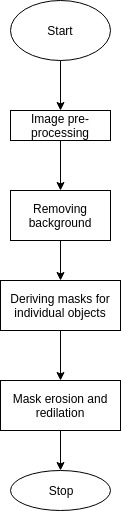
\includegraphics[height=12cm, width=.5\linewidth]{flw.jpg}
\caption{Flowchart of the procedure followed}
\label{fig:FMI_Cancer_Cell_Line}
\end{figure}

\subsection{Image pre-processing}
Broadly speaking, there are three types of cell segmentation techniques namely: feature based, model based and learning based. Since we are doing this to learn classical image processing, we will not touch learning based techniques here.
Since single channel microscopy presents more complexities, we are using multi-channel data set acquired in Biotechnology Department. The images samples of cell can be of any of the color formats, based on the illumination conditions and type of microscope with which they were acquired. 

\begin{figure}
\centering
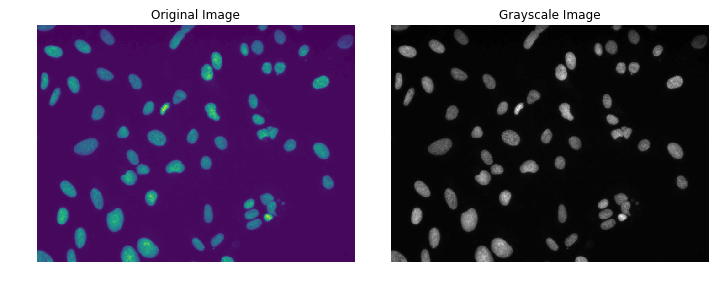
\includegraphics[width=.9\linewidth]{original_n_greyscale.png}
\caption{Original (left) and converted grayscale (right) image}
\label{fig:greyscale}
\end{figure}
 
 \subsection{Removing background}
We found that there are two classes in the image: objects of interest and the background. Under this assumption, we would expect the data to fall into a bimodal distribution of intensities. If we found the best separation value, we could "mask" out the background data, then simply count the objects we're left with.

We can find the optimal threshold value using the Otsu's thresholding method by assuming image as bimodal image distribution.

\subsection{Deriving masks for individual objects}
We look for all objects in the mask that are connected, and assign each of them a number. Then, we can loop through each and add it to an iterable, such as an array.
We found that some adjacent cells are combined into a single cell. We could iterate through our masks, zooming in on the individual nuclei which found with need to apply additional processing steps.  Then, we find out the coordinate range for each labeled object in our image.

\subsection{Mask erosion and dilation}
 Many labels have the "adjacent cell" problem: the two cells are being considered part of the same object. One thing we can do here is to see whether we can shrink the mask to "open up" the differences between the cells. This is called mask erosion. We can then re-dilate it to to recover the original proportions.


\section{Results}
We have implemented the operations mentioned above in the images. Fig \ref{fig:greyscale} shows the conversion of color images to grayscale. 


\begin{figure}
\centering
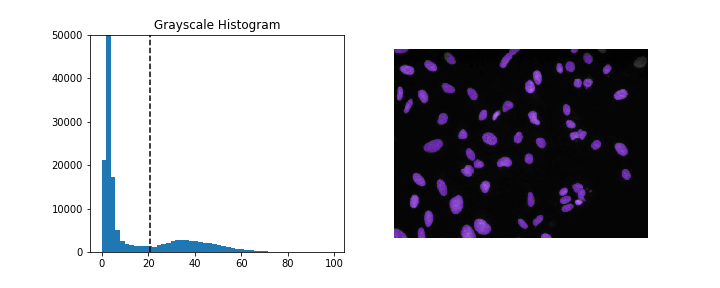
\includegraphics[height=6cm, width=1.145\linewidth]{hist.png}
\caption{Histogram of the grayscale image}
\label{fig:hist}
\end{figure}


Fig \ref{fig:hist} shows the image with binary mask after Otsu's thresholding as well as the histogram showing the intensity threshold.

\begin{figure}
\centering
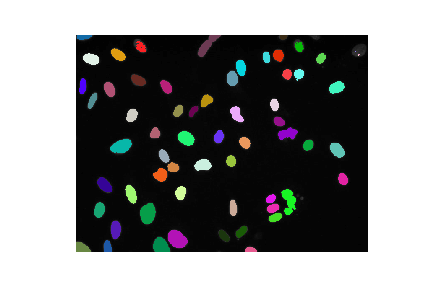
\includegraphics[height=6cm, width=1.145\linewidth]{labelled_cells.png}
\caption{Labelled Cells}
\label{fig:label}
\end{figure}

Fig \ref{fig:label} shows the labelled images to which morphological opening operation will be performed. Fig \ref{fig:indiLabel} shows the individual labelled cells. In case of overlapping cells, we 

\begin{figure}
\centering
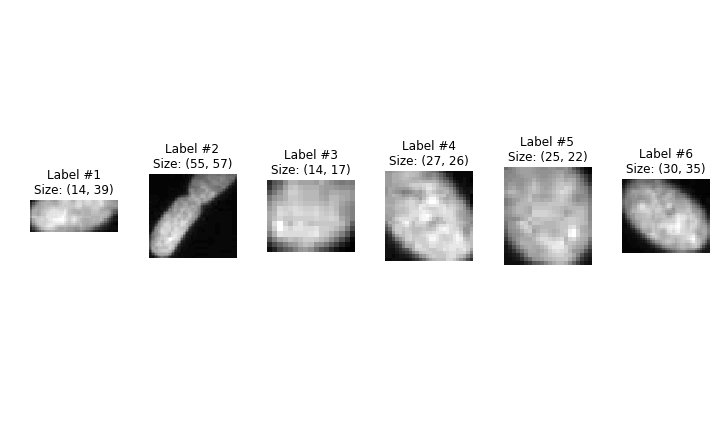
\includegraphics[height=6cm, width=\linewidth]{indiLabel.png}
\caption{Individual labelled images}
\label{fig:indiLabel}
\end{figure}

\begin{figure}
\centering
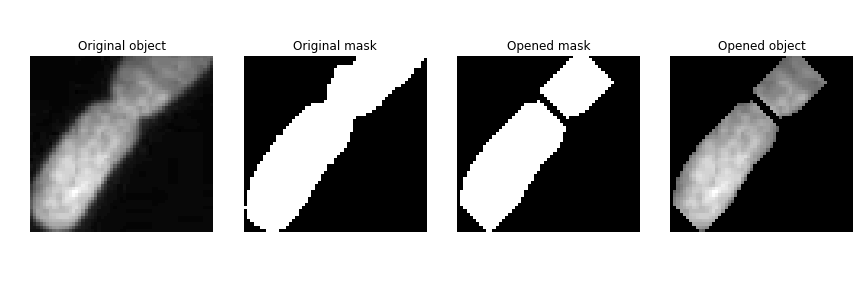
\includegraphics[height=6cm, width=\linewidth]{mask.png}
\caption{Morphological opening procedure}
\label{fig:label}
\end{figure}




% use this to cite image
% \ref{fig:labelledCells}


% use this to cite image
% \ref{fig:label}

For the above image, the number of objects/nuclei detected are 60. Manually, the count observed is 63. Therefore, the efficiency is around 96 percent.

\section{CONCLUSION}
Using thresholding operation, we have labelled the segmented cells with reasonable accuracy. Therefore the above classical image processing technique as shown can be used often to segment the cells, works reasonably better than watershed and hence have a wide application in biomedical image analysis.


\begin{thebibliography}{99}

\bibitem{c1} D. Liu and J. Yu, "Otsu Method and K-means," 2009 Ninth International Conference on Hybrid Intelligent Systems, Shenyang, 2009, pp. 344-349.
\bibitem{c2} X. Cui, Y. Deng, G. Yang and S. Wu, "An improved image segmentation algorithm based on the watershed transform," 2014 IEEE 7th Joint International Information Technology and Artificial Intelligence Conference, Chongqing, 2014, pp. 428-431.
\bibitem{c3} 

\end{thebibliography}
\end{document}
